\section{Ejercicio 1}

$$
F(x,y,z) = \sum(2,3,4,5)
$$

\subsection{Expresión mínima}

\begin{figure}[H]
    \centering
    \begin{karnaugh-map}[2][4][1][$z$][$y$][$x$]
        \centering
        \minterms{2,3,4,5}
        \implicant{2}{3}
        \implicant{4}{5}
    \end{karnaugh-map}
    \caption{Mapa de Karnaugh para la función}
\end{figure}

$$
F(x,y,z) = x \overline{y} + \overline{x} y
$$

\subsection{Simulación en Falstad}
\begin{figure}[H]
    \centering
    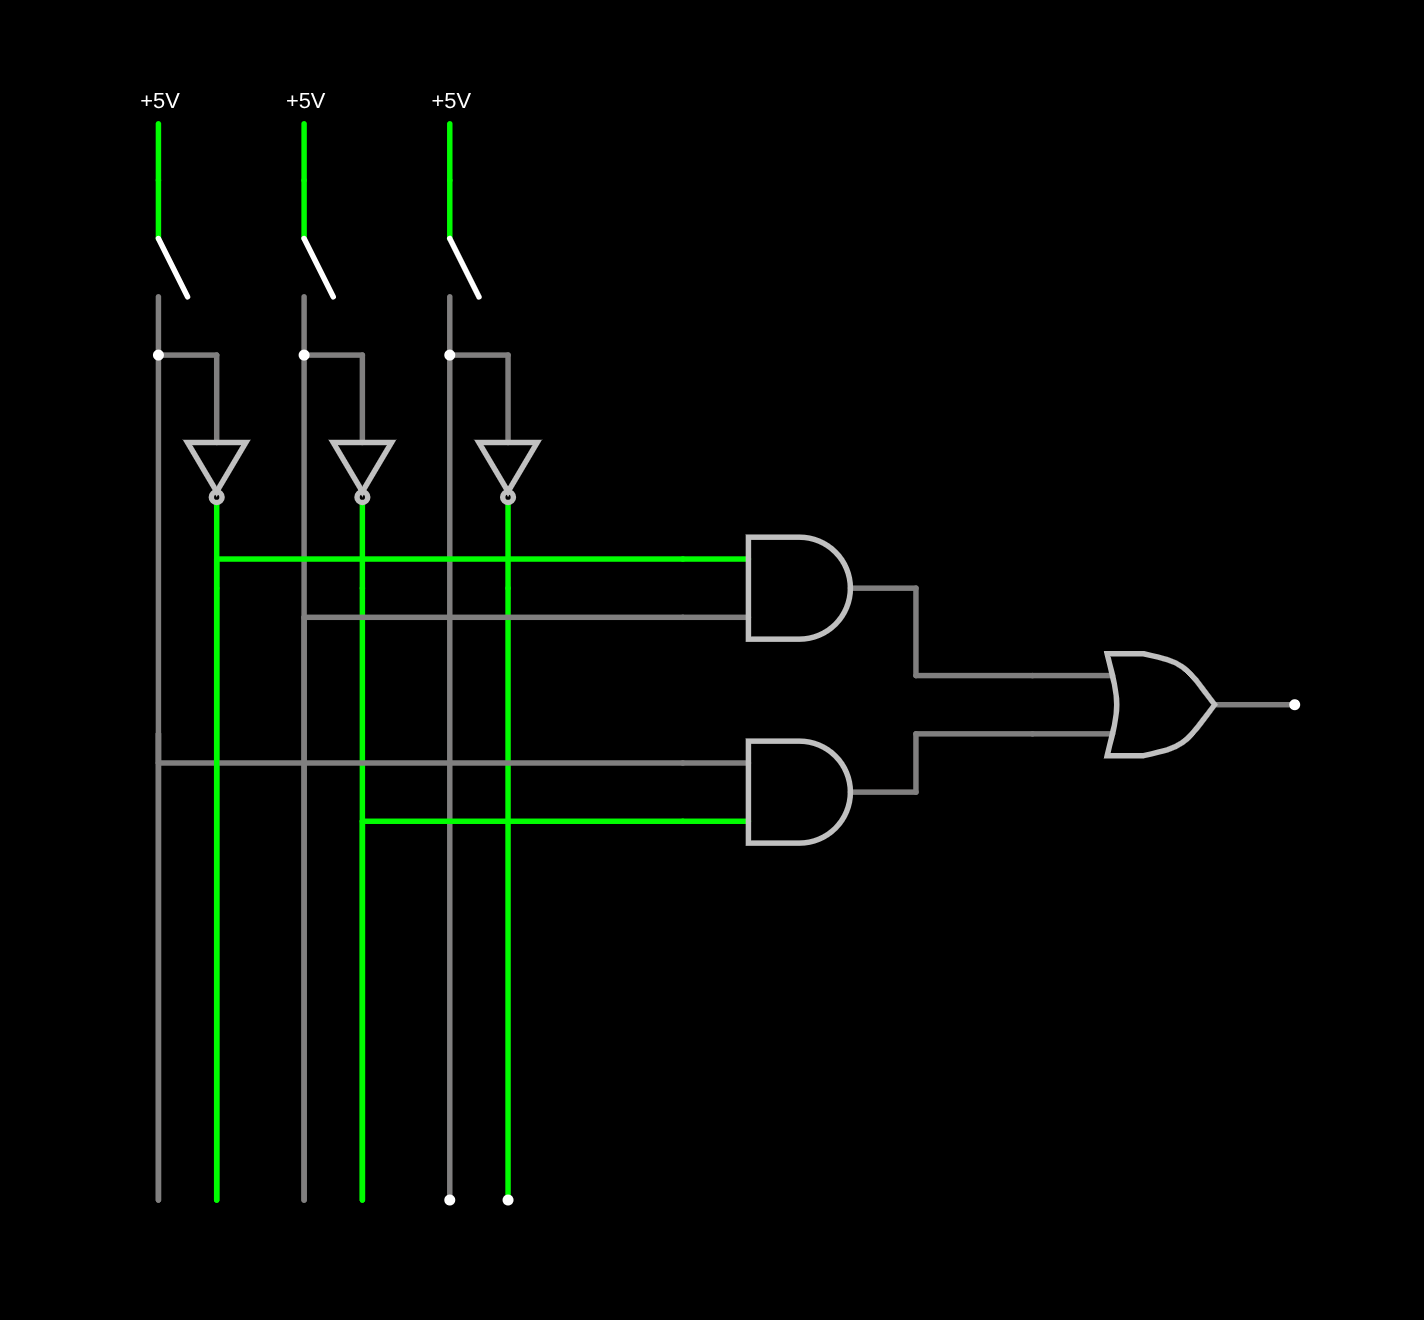
\includegraphics[width=0.6\textwidth]{img/Falstad/ej1.png}
    \caption{Simulación de la función en Falstad}
\end{figure}

\subsection{Descripción en Verilog}

\begin{Verbatim}[ frame=single, fontsize=\small, baselinestretch=1.2 ]
module ej1 (
    input x,
    input y,
    input z,
    output F
);

assign F = x & ~y | ~x & y;

endmodule
\end{Verbatim}

\subsection{Captura del RTL}
\begin{figure}[H]
    \centering
    
\includegraphics[width=0.8\textwidth]{img/Xilinx/ej1.png}
    \caption{Captura del RTL en Xilinx}
\end{figure}